\documentclass[12pt]{article}
\usepackage[a4paper, margin=.30in]{geometry}
\usepackage{graphicx ,
            wrapfig,
            xcolor, 
            enumerate,
            amsmath,fontenc,mathrsfs,makecell
            }

\newcommand\headerMe[2]{\noindent{}#1\hfill#2}
\renewcommand{\thesection}{\Roman{section}}

\title{Leçon N 7 :Equilibre d’un solide en rotation autour d’un axe fixe }
\author{Zakaria HAOUZAN}
\date{\today}

\begin{document}
% headers --------------
\headerMe{Matière : Physique-Chimie}{Professeur : Zakaria HAOUZAN}\\
\headerMe{Unité : La Mécanique}{Établissement : Lycée SKHOR qualifiant}\\
\headerMe{Niveau : TCS}{Heure : 3H}\\

% ------Content ________
\begin{center}
    \Large{Leçon $N^{\circ}7$: \color{red}Equilibre d’un solide en rotation autour d’un axe fixe }
\end{center}

\begin{wrapfigure}{r}{0.2\textwidth}
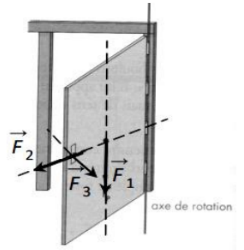
\includegraphics[width=0.2\textwidth]{./img/img_00.png}
%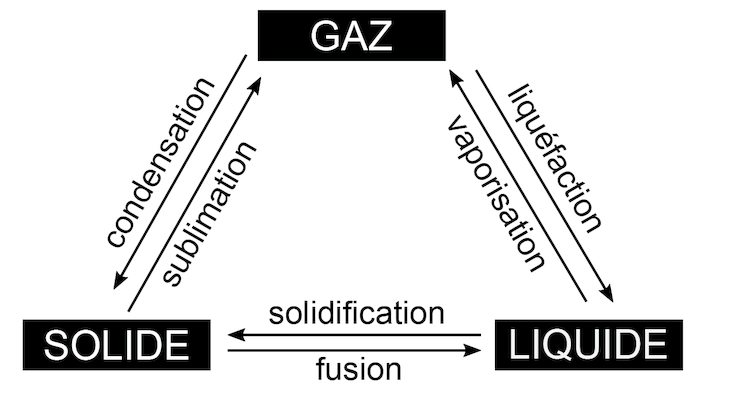
\includegraphics[width=0.2\textwidth]{./img/img01.jpg}
\end{wrapfigure}



\section{Effet d’une force sur la rotation d’un solide : }
-si on exerce sur une porte ouverte une force F1 parallèle à l'axe de rotation, celle-ci ne tourne pas.

-si on exerce sur cette porte une force F2 dont la droite d action coupe l'axe, elle ne tourne pas non plus

-une force F3 perpendiculaire à l'axe de rotation provoque une rotation. 
L'efficacité de la rotation dépend de l'intensité de la force et de la position de la droite d'action, par rapport à l'axe de rotation.




\section{Moment d'une force par rapport à un axe : }
\subsection{Définition du moment d une force : }
Le moment d'une force par rapport à un axe traduit son efficacité à produire un effet de rotation du solide autour de cet axe .

L'intensité du moment par rapport à un axe d'une force $\vec{F}$orthogonale à cet axe est :$$\mathscr{M}(\vec{F}) = \pm F.d$$ 
\begin{center}
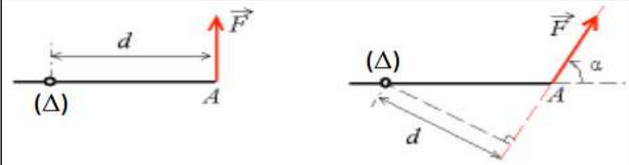
\includegraphics[width=0.5\textwidth]{./img/img_01.png}
\end{center}
\begin{center}
\begin{tabular}{ |c|c|  }
 \hline
 \multicolumn{2}{|c|}
  {\makecell{
Afin de distinguer les deux possibilités de sens de rotation nous évaluerons algébriquement \\le moment d'une force par rapport à l'axe par l une des expressions suivantes:
  }} \\
 \hline
  \makecell{lorsque F tend à faire tourner le solide dans le sens\\ positif choisi} &
  \makecell{lorsque F tend à faire tourner le solide dans le sens\\
contraire au sens positif choisi }\\
 \hline
  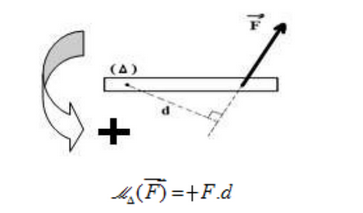
\includegraphics[width=0.4\textwidth]{./img/img_03.png} 

  & 
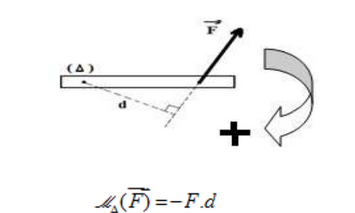
\includegraphics[width=0.4\textwidth]{./img/img_02.png}\\

 \hline
\end{tabular}
\end{center}

\section{Théorème des moments:}
Lorsqu un solide, mobile autour d'un axe fixe, est en équilibre, la somme algébrique des moments, par rapport à cet axe
$$\sum\mathscr{M}_{\Delta}(\vec{F}_{ext}) = \vec{0}$$

\vspace{0.2cm}
REMARQUE : Conditions générales d'équilibre
Lorsque un solide est en équilibre, deux conditions doivent être satisfaites.

-$\sum{\vec{F_{ext}}} = \vec{0}$

-$\sum\mathscr{M}_{\Delta}(\vec{F}_{ext}) = \vec{0}$
\section{Couples de forces : }
\subsection{Définition d un couple de forces : }

Un couple de force est un système de deux forces parallèles, de sens contraires, de même intensité et n'ayant
pas la même droite support((lignes d'action différentes)

\subsection{Moment d un couple de forces : }
Le moment d un couple de force ne dépend pas de la position de l axe de rotation mais seulement de
distante des deux lignes d action.

$\mathscr{M}_{\Delta}(C) = \mathscr{M}_{\Delta}(\vec{F}_1) + \mathscr{M}_{\Delta}(\vec{F}_2) = F_1.d_1 + F_2.d_2$

avec $F_1 = F_2 = F$ et $d_1 + d_2 = d$ d est la distance séparant les deux droites d action.
$$
  \mathscr{M}_\Delta = F.d
$$
En générale Le moment d un couple de force est : $\mathscr{M}_\Delta =\pm F.d$
\section{Couple de torsion : }

Un pendule de torsion est un solide suspendu à un fil vertical, le centre de masse étant sur l'axe du fil, l'autre
extrémité du fil étant maintenue fixe dans un support.

Quand le solide tourne autour de l'axe du fil, celui-ci réagit à la torsion en exerçant des forces de rappel équivalentes à un couple dont le moment par rapport à l'axe est proportionnel à l'angle de torsion $\theta$en (rad) :
$$
\mathscr{M}_\Delta =-C.\theta
$$
\begin{center}
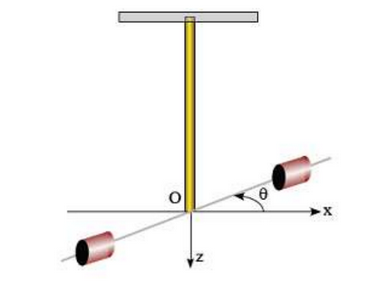
\includegraphics[width=0.4\textwidth]{./img/img_04.png}\\
\end{center}
La constante C dite constante de torsion dépend de la longueur et du diamètre du fil (supposé cylindrique) et
de la nature du matériau constituant le fil en N.m/rad.
\end{document}
